% Meridian Capital, Round 2. Compile twice with XeLaTeX.
\documentclass[aspectratio=169,11pt,t]{beamer}
\usepackage{lmodern}
\usepackage{fontspec}
\setmainfont{DMSans-Regular.ttf}[BoldFont=DMSans-Bold.ttf,ItalicFont=DMSans-Italic.ttf,BoldItalicFont=DMSans-BoldItalic.ttf]
\setsansfont{DMSans-Regular.ttf}[BoldFont=DMSans-Bold.ttf,ItalicFont=DMSans-Italic.ttf,BoldItalicFont=DMSans-BoldItalic.ttf]
\usefonttheme{professionalfonts}
\usepackage{microtype,booktabs,array,tabularx,graphicx,tikz,appendixnumberbeamer}
\usetikzlibrary{calc}
\definecolor{navy}{HTML}{0A2233}
\definecolor{ink}{HTML}{173242}
\definecolor{gold}{HTML}{A59577}
\definecolor{paper}{HTML}{F7F5EF}
\definecolor{muted}{HTML}{59666B}
\definecolor{line}{HTML}{D9DCD7}
\definecolor{loss}{HTML}{8F4E3A}
\usetheme{default}
\setbeamercolor{normal text}{fg=ink,bg=white}
\setbeamercolor{structure}{fg=navy}
\setbeamercolor{frametitle}{fg=navy}
\setbeamercolor{itemize item}{fg=gold}
\setbeamertemplate{itemize item}[square]
\setbeamertemplate{navigation symbols}{}
\setbeamersize{text margin left=1.05cm,text margin right=1.05cm}
\setbeamerfont{normal text}{size=\normalsize}
\setbeamertemplate{frametitle}{%
  \vspace{.35cm}\nointerlineskip
  \begin{beamercolorbox}[wd=\textwidth,sep=0pt]{frametitle}
  {\fontsize{20}{24}\selectfont\insertframetitle\par}
  \vspace{.10cm}{\color{gold}\rule{\linewidth}{.7pt}}
  \end{beamercolorbox}\vspace{.14cm}}
\setbeamertemplate{footline}{%
  \hspace{1.05cm}\begin{minipage}{\dimexpr\paperwidth-2.1cm\relax}
  {\color{line}\hrule height .3pt}\vspace{3pt}
  {\fontsize{5.7}{7}\selectfont\color{muted}MERIDIAN CAPITAL\enspace ·\enspace AMC 2026
  \hfill\insertframenumber\,/\,\inserttotalframenumber}\vspace{5pt}
  \end{minipage}}
\newcommand{\source}[1]{\par\vfill{\fontsize{6.3}{8}\selectfont\color{muted}#1\par}}
\newcommand{\reportsection}[1]{\href{https://kybeka.github.io/meridian-capital/materials/round-2-report.pdf}{Submitted report, #1}}
\newcommand{\labeltext}[1]{{\fontsize{8}{10}\selectfont\color{gold}\textbf{#1}}}
\newcommand{\bigvalue}[1]{{\fontsize{29}{33}\selectfont\color{navy}#1}}
\newcommand{\point}[2]{\textbf{#1}\par\vspace{.04cm}#2\par\vspace{.12cm}}
\newcommand{\smallnote}[1]{{\fontsize{8}{10}\selectfont\color{muted}#1}}
\newcommand{\tablefont}{\fontsize{9}{11.5}\selectfont}
\hypersetup{colorlinks=true,urlcolor=muted,linkcolor=navy}
\pdfstringdefDisableCommands{\def\translate#1{#1}}
\begin{document}
{
\setbeamertemplate{footline}{}
\setbeamercolor{background canvas}{bg=paper}
\begin{frame}[plain]
\centering
\vspace{.18cm}

\includegraphics[width=4.4cm]{Meridian-Capital-Official-Logo.png}\par
\vspace{.10cm}{\color{gold}\rule{3cm}{.8pt}}\par\vspace{.20cm}
{\fontsize{25}{29}\selectfont\color{navy}Tactical Deviation\par}
\vspace{.13cm}{\large Discretionary equity investing\par}
\vspace{.22cm}{\small\color{muted}One-third of the portfolio in six stocks\par}
\vfill
{\fontsize{8}{11}\selectfont Alessia Battistella\enspace ·\enspace Tze Qing Ginnie Lee\enspace ·\enspace Katherine Lerner-Teves\\
Kyla Kaplan\enspace ·\enspace Lorenzo Comi\par}
\vspace{.18cm}{\fontsize{7}{9}\selectfont\color{muted}USI\enspace ·\enspace Asset Management Challenge 2026\enspace ·\enspace Round 2\par}
\vspace{.18cm}
\note{We put one-third of the portfolio into six stocks. We'll start with how Round 1 went, then explain the companies, the weights and the risks. We still use our original ETF allocation as the benchmark.}
\end{frame}}

\begin{frame}{Round 1 performance}

\begin{columns}[T,onlytextwidth]
\begin{column}{.42\textwidth}
\labeltext{16 OCTOBER--6 NOVEMBER}\par\vspace{.12cm}
\bigvalue{−2.885\%}\par\small Ending NAV: \$97.115m\par\vspace{.35cm}
\begin{tabular}{@{}lr@{}}\toprule
Realized volatility & 8.14\%\\
SAA target & 8.00\%\\
Realized Sharpe & $-6.50$\\\bottomrule
\end{tabular}\par\vspace{.25cm}
\smallnote{With only fifteen daily returns, a few losses have a large effect on annualized Sharpe.}
\end{column}
\begin{column}{.53\textwidth}
\labeltext{CONTRIBUTION TO RETURN, PP}\par\vspace{.12cm}
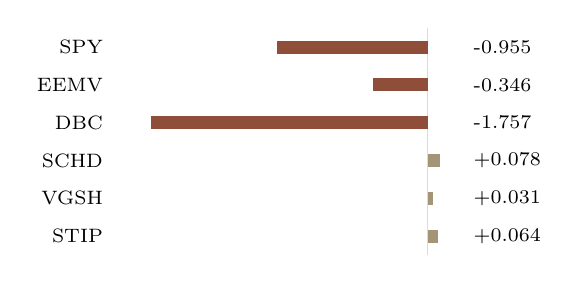
\begin{tikzpicture}[x=2.0cm,y=.48cm]\draw[line] (0,.5)--(0,-5.5);\node[anchor=east,font=\scriptsize] at (-2.0,0) {SPY};\fill[loss] (0,-0.17) rectangle (-0.955365,0.17);\node[anchor=west,font=\scriptsize] at (.23,0) {-0.955};\node[anchor=east,font=\scriptsize] at (-2.0,-1) {EEMV};\fill[loss] (0,-1.17) rectangle (-0.34605,-0.83);\node[anchor=west,font=\scriptsize] at (.23,-1) {-0.346};\node[anchor=east,font=\scriptsize] at (-2.0,-2) {DBC};\fill[loss] (0,-2.17) rectangle (-1.757263,-1.83);\node[anchor=west,font=\scriptsize] at (.23,-2) {-1.757};\node[anchor=east,font=\scriptsize] at (-2.0,-3) {SCHD};\fill[gold] (0,-3.17) rectangle (0.0783,-2.83);\node[anchor=west,font=\scriptsize] at (.23,-3) {+0.078};\node[anchor=east,font=\scriptsize] at (-2.0,-4) {VGSH};\fill[gold] (0,-4.17) rectangle (0.031106,-3.83);\node[anchor=west,font=\scriptsize] at (.23,-4) {+0.031};\node[anchor=east,font=\scriptsize] at (-2.0,-5) {STIP};\fill[gold] (0,-5.17) rectangle (0.064341,-4.83);\node[anchor=west,font=\scriptsize] at (.23,-5) {+0.064};\end{tikzpicture}
\par\vspace{.16cm}\textbf{DBC accounts for 61\% of the net loss.}
\end{column}\end{columns}
\source{Closing prices, including \$100,916.79 of VGSH/STIP distributions in NAV. \reportsection{4}.}

\note{We lost 2.885 percent in Round 1, leaving about 97.115 million dollars. DBC caused most of the loss: minus 1.757 percentage points, or about 61 percent of the total. SPY was the next-largest loss. Realized volatility was 8.14 percent, close to our 8 percent target. Sharpe was minus 6.50, but that comes from only fifteen daily returns. Both ETF distributions are included in NAV.}
\end{frame}

\begin{frame}{How we paid for the stocks}


\begin{tikzpicture}[x=1cm,y=1cm]
\fill[gold] (0,0) rectangle (9.1,.7);\fill[navy] (9.1,0) rectangle (13.65,.7);
\node[text=white,font=\bfseries] at (4.55,.35) {66.67\% original ETFs};
\node[text=white,font=\bfseries] at (11.375,.35) {33.33\% stocks};
\end{tikzpicture}\par\vspace{.20cm}
\begin{columns}[T,onlytextwidth]
\begin{column}{.48\textwidth}\tablefont
\begin{tabular}{@{}lrr@{}}\toprule ETF & SAA & Round 2 target\\\midrule
SPY&26.08\%&17.39\%\\
EEMV&9.66\%&6.44\%\\
DBC&26.95\%&17.97\%\\
SCHD&3.28\%&2.19\%\\
VGSH&5.00\%&3.33\%\\
STIP&29.03\%&19.35\%\\
\bottomrule\end{tabular}
\end{column}
\begin{column}{.46\textwidth}
\point{\$32.372m stock budget}{One-third of the portfolio value after Round 1, as required in class.}
\point{Sell each ETF proportionally}{We reduce each ETF target to two-thirds of its original weight.}
\smallnote{DBC falls from 26.95\% to 17.97\%. Exxon also exposes us to energy prices.}
\end{column}\end{columns}
\source{NAV \$97,115,068.58. Entered 7 November using 6 November closing prices. No fees; whole-share cash \$116.05. \reportsection{1.1 and 5}.}

\note{The class instruction was to put one-third into stocks. We decided to fund that by reducing each ETF target to two-thirds of its original weight. This keeps the relative ETF mix the same. We used the portfolio value after the Round 1 loss and distributions. That gave us a stock budget of about 32.372 million dollars. After rounding and the extra SPY and Adobe shares, we have 116.05 dollars in cash.}
\end{frame}

\begin{frame}{How we valued the stocks}

\begin{center}{\large\color{navy}Normalized EPS $\times$ our chosen P/E = estimated value}\end{center}
\vspace{.10cm}\tablefont
\begin{tabularx}{\textwidth}{@{}Xrrrrr@{}}\toprule
Stock & Entry price & EPS & P/E & Value & Margin of safety\\\midrule
ADBE&\$239.30&18.145&16$\times$&\$290.32&17.57\%\\
KR&\$67.70&5.2&15$\times$&\$78.00&13.21\%\\
HRL&\$21.95&1.48&17$\times$&\$25.16&12.76\%\\
BMY&\$62.14&6.45&11$\times$&\$70.95&12.42\%\\
XOM&\$165.87&10&18$\times$&\$180.00&7.85\%\\
HPQ&\$28.46&2.38&13.5$\times$&\$32.13&11.42\%\\
\bottomrule\end{tabularx}\par\vspace{.33cm}
\begin{columns}[T,onlytextwidth]
\begin{column}{.48\textwidth}\point{Are the earnings sustainable?}{We check guidance, one-off items, cash flow and peers.}\end{column}
\begin{column}{.48\textwidth}\point{What could change the price?}{We check cash values, business risks and news expected before the challenge ends.}\end{column}
\end{columns}
\source{USD per share. Margin of safety = $1-P/V$; upside = $V/P-1$. EPS basis differs by company and is stated on each stock slide. \reportsection{2 and 3}.}

\note{For each company, we chose an earnings figure and a P/E multiple, then checked the value against cash flow. We also looked for news that could affect the price before the challenge ends. Adobe and HP use GAAP earnings. Kroger, Hormel and BMY use adjusted guidance. Exxon's ten-dollar EPS is our estimate across the cycle. Margin of safety measures the discount relative to our value; upside measures it relative to the entry price.}
\end{frame}

\begin{frame}{ADBE | Adobe}

\begin{columns}[T,onlytextwidth]
\begin{column}{.34\textwidth}
\labeltext{NAV ALLOCATION}\par\vspace{.08cm}\bigvalue{4.65\%}\par\vspace{.27cm}
\textbf{Earnings value: \$290.32}\par\vspace{.08cm}
\smallnote{GAAP EPS \$18.145 $\times$ 16}\par\vspace{.28cm}
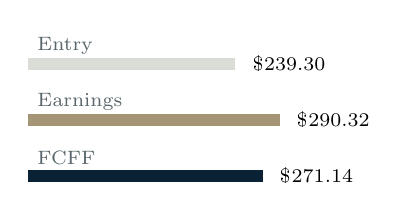
\begin{tikzpicture}[x=1cm,y=.62cm]\node[anchor=west,font=\scriptsize,text=muted]at(0,0.37){Entry};\fill[line](0,-0.13)rectangle(2.637641223477542,0.12);\node[anchor=west,font=\scriptsize]at(2.7376412234775422,0.0){\$239.30};\node[anchor=west,font=\scriptsize,text=muted]at(0,-0.7799999999999999){Earnings};\fill[gold](0,-1.2799999999999998)rectangle(3.2,-1.0299999999999998);\node[anchor=west,font=\scriptsize]at(3.3000000000000003,-1.15){\$290.32};\node[anchor=west,font=\scriptsize,text=muted]at(0,-1.9299999999999997){FCFF};\fill[navy](0,-2.4299999999999997)rectangle(2.988615935263681,-2.1799999999999997);\node[anchor=west,font=\scriptsize]at(3.088615935263681,-2.3){\$271.14};\end{tikzpicture}
\par\vspace{.16cm}\smallnote{Earnings margin of safety: 17.57\%}
\end{column}
\begin{column}{.62\textwidth}
\point{Strong cash flow, with AI competition to watch}{FCF margin is 41.4\%, above history and peers. Cash values deduct SBC.}
\point{Catalyst}{\textbf{9 December:} FY2027 outlook on renewals, prices and paid AI revenue.}
\point{Main risk}{Customers may switch to cheaper AI tools. A 20\% cash reduction gives a value of \$216.54.}
\end{column}\end{columns}
\source{USD per share. Cash values use our FCFF assumptions. \reportsection{2.1}; \href{https://www.sec.gov/Archives/edgar/data/796343/000079634326000147/adbeex991q326.htm}{issuer earnings release}.}

\note{We chose Adobe because its subscription business generates a lot of cash and our earnings value is above the entry price. We use GAAP EPS, which includes stock compensation. The cash model gives a lower value, still above entry. The main concern is whether cheaper AI tools lead customers to leave or pay less. On December 9, we'll look at renewals, pricing and revenue from paid AI features. In our stress test, a twenty-percent cash reduction takes value below entry.}
\end{frame}

\begin{frame}{KR | Kroger}

\begin{columns}[T,onlytextwidth]
\begin{column}{.34\textwidth}
\labeltext{NAV ALLOCATION}\par\vspace{.08cm}\bigvalue{8.10\%}\par\vspace{.27cm}
\textbf{Earnings value: \$78.00}\par\vspace{.08cm}
\smallnote{Adjusted EPS \$5.20 $\times$ 15}\par\vspace{.28cm}
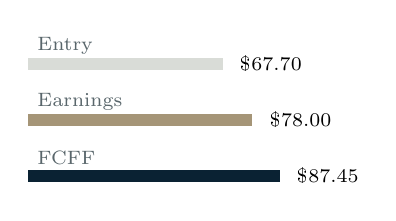
\begin{tikzpicture}[x=1cm,y=.62cm]\node[anchor=west,font=\scriptsize,text=muted]at(0,0.37){Entry};\fill[line](0,-0.13)rectangle(2.4772607683072785,0.12);\node[anchor=west,font=\scriptsize]at(2.5772607683072786,0.0){\$67.70};\node[anchor=west,font=\scriptsize,text=muted]at(0,-0.7799999999999999){Earnings};\fill[gold](0,-1.2799999999999998)rectangle(2.8541556857897743,-1.0299999999999998);\node[anchor=west,font=\scriptsize]at(2.9541556857897744,-1.15){\$78.00};\node[anchor=west,font=\scriptsize,text=muted]at(0,-1.9299999999999997){FCFF};\fill[navy](0,-2.4299999999999997)rectangle(3.2,-2.1799999999999997);\node[anchor=west,font=\scriptsize]at(3.3000000000000003,-2.3){\$87.45};\end{tikzpicture}
\par\vspace{.16cm}\smallnote{Earnings margin of safety: 13.21\%}
\end{column}
\begin{column}{.62\textwidth}
\point{Steady grocery demand and good cash conversion}{FCF margin is 2.3\%, above history and peers. Grocery margins are thin.}
\point{Catalyst}{\textbf{3 December:} results after the e-commerce reset: sales, fulfillment costs and guidance.}
\point{Main risk}{Cash covers dividends 2.40$\times$. Buybacks exceed the cash left after dividends.}
\end{column}\end{columns}
\source{USD per share. Cash values use our FCFF assumptions. \reportsection{2.2}; \href{https://ir.kroger.com/news/news-details/2026/Kroger-Reports-Second-Quarter-2026-Results-and-Updates-Guidance-for-2026/default.aspx}{issuer earnings release}.}

\note{Kroger sells groceries, so demand is fairly steady. Its FCF margin is also above its recent history and peers. We use adjusted earnings because the fulfillment charges distort GAAP EPS. The December results should help us assess sales and costs after the e-commerce reset. Dividends are covered, but buybacks are larger than the cash left over. We want to see enough cash from the business to support those payouts.}
\end{frame}

\begin{frame}{HRL | Hormel Foods}

\begin{columns}[T,onlytextwidth]
\begin{column}{.34\textwidth}
\labeltext{NAV ALLOCATION}\par\vspace{.08cm}\bigvalue{6.90\%}\par\vspace{.27cm}
\textbf{Earnings value: \$25.16}\par\vspace{.08cm}
\smallnote{Adjusted EPS \$1.48 $\times$ 17}\par\vspace{.28cm}
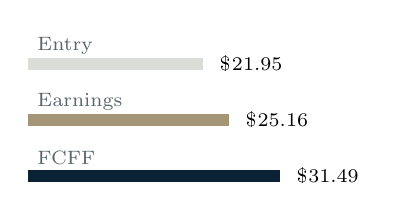
\begin{tikzpicture}[x=1cm,y=.62cm]\node[anchor=west,font=\scriptsize,text=muted]at(0,0.37){Entry};\fill[line](0,-0.13)rectangle(2.2306712391462855,0.12);\node[anchor=west,font=\scriptsize]at(2.3306712391462856,0.0){\$21.95};\node[anchor=west,font=\scriptsize,text=muted]at(0,-0.7799999999999999){Earnings};\fill[gold](0,-1.2799999999999998)rectangle(2.5568878531626673,-1.0299999999999998);\node[anchor=west,font=\scriptsize]at(2.6568878531626674,-1.15){\$25.16};\node[anchor=west,font=\scriptsize,text=muted]at(0,-1.9299999999999997){FCFF};\fill[navy](0,-2.4299999999999997)rectangle(3.2,-2.1799999999999997);\node[anchor=west,font=\scriptsize]at(3.3000000000000003,-2.3){\$31.49};\end{tikzpicture}
\par\vspace{.16cm}\smallnote{Earnings margin of safety: 12.76\%}
\end{column}
\begin{column}{.62\textwidth}
\point{Margins and cash flow need to recover}{We need margins to recover to justify 17$\times$ earnings. FCF margin is only 4.4\%.}
\point{Catalyst}{\textbf{3 December:} the new CEO's FY2027 outlook. We will watch Retail volumes and margins.}
\point{Main risk}{Dividend cover falls from 1.17$\times$ to about 1.00$\times$ with acquisition debt and refinancing costs.}
\end{column}\end{columns}
\source{USD per share. Cash values use our FCFF assumptions. \reportsection{2.3}; \href{https://www.hormelfoods.com/wp-content/uploads/Hormel-Earnings-Release-Q3-2026_FINAL.pdf}{issuer earnings release}.}

\note{Hormel needs its margins and cash flow to recover. Our P/E is above the food peers we used, so the December outlook needs to support that choice. We'll watch Retail volumes, earnings guidance and dividend coverage. Buying Brakebush requires cash and new debt, while the earnings benefit is expected only from fiscal 2028. In the combined debt and refinancing stress, dividend coverage falls to about one time. That leaves very little room for a disappointment.}
\end{frame}

\begin{frame}{BMY | Bristol Myers Squibb}

\begin{columns}[T,onlytextwidth]
\begin{column}{.34\textwidth}
\labeltext{NAV ALLOCATION}\par\vspace{.08cm}\bigvalue{6.33\%}\par\vspace{.27cm}
\textbf{Earnings value: \$70.95}\par\vspace{.08cm}
\smallnote{Non-GAAP EPS \$6.45 $\times$ 11}\par\vspace{.28cm}
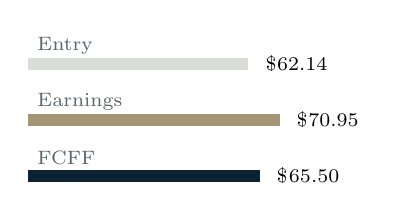
\begin{tikzpicture}[x=1cm,y=.62cm]\node[anchor=west,font=\scriptsize,text=muted]at(0,0.37){Entry};\fill[line](0,-0.13)rectangle(2.8026497533474277,0.12);\node[anchor=west,font=\scriptsize]at(2.902649753347428,0.0){\$62.14};\node[anchor=west,font=\scriptsize,text=muted]at(0,-0.7799999999999999){Earnings};\fill[gold](0,-1.2799999999999998)rectangle(3.2,-1.0299999999999998);\node[anchor=west,font=\scriptsize]at(3.3000000000000003,-1.15){\$70.95};\node[anchor=west,font=\scriptsize,text=muted]at(0,-1.9299999999999997){FCFF};\fill[navy](0,-2.4299999999999997)rectangle(2.954116495127397,-2.1799999999999997);\node[anchor=west,font=\scriptsize]at(3.054116495127397,-2.3){\$65.50};\end{tikzpicture}
\par\vspace{.16cm}\smallnote{Earnings margin of safety: 12.42\%}
\end{column}
\begin{column}{.62\textwidth}
\point{New medicines need to replace lost sales}{We use 11$\times$ earnings and flat cash flow to allow for patent expiries.}
\point{Catalyst}{\textbf{12--15 December:} ASH data. Milvexian/Sotyktu results are expected by year-end; exact dates are unknown.}
\point{Main risk}{There is little room for weaker cash flow. A 2\% annual decline for five years gives \$58.59.}
\end{column}\end{columns}
\source{USD per share. Cash values use our FCFF assumptions. \reportsection{2.4}; \href{https://www.bms.com/assets/bms/us/en-us/pdf/investor-info/doc_financials/quarterly_reports/2026/BMY-Q3-2026-Earnings-Press-Release-0039.pdf}{issuer earnings release}.}

\note{BMY needs new medicines to replace sales lost when patents expire. We use a low earnings multiple and assume flat cash flow. That cash model gives 65.50 dollars, quite close to the entry price. We kept the disclosed research and licensing costs in earnings. ASH has fixed December dates, but the major trial results have no confirmed day and could miss the cutoff. A two-percent annual cash decline already takes value below entry, so the pipeline results matter a lot.}
\end{frame}

\begin{frame}{XOM | Exxon Mobil}

\begin{columns}[T,onlytextwidth]
\begin{column}{.34\textwidth}
\labeltext{NAV ALLOCATION}\par\vspace{.08cm}\bigvalue{3.62\%}\par\vspace{.27cm}
\textbf{Earnings value: \$180.00}\par\vspace{.08cm}
\smallnote{Cycle-normalized EPS \$10.00 $\times$ 18}\par\vspace{.28cm}
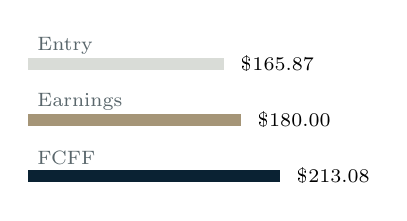
\begin{tikzpicture}[x=1cm,y=.62cm]\node[anchor=west,font=\scriptsize,text=muted]at(0,0.37){Entry};\fill[line](0,-0.13)rectangle(2.4909591988106263,0.12);\node[anchor=west,font=\scriptsize]at(2.5909591988106264,0.0){\$165.87};\node[anchor=west,font=\scriptsize,text=muted]at(0,-0.7799999999999999){Earnings};\fill[gold](0,-1.2799999999999998)rectangle(2.7031570252963935,-1.0299999999999998);\node[anchor=west,font=\scriptsize]at(2.8031570252963935,-1.15){\$180.00};\node[anchor=west,font=\scriptsize,text=muted]at(0,-1.9299999999999997){FCFF};\fill[navy](0,-2.4299999999999997)rectangle(3.1999999999999997,-2.1799999999999997);\node[anchor=west,font=\scriptsize]at(3.3,-2.3){\$213.08};\end{tikzpicture}
\par\vspace{.16cm}\smallnote{Earnings margin of safety: 7.85\%}
\end{column}
\begin{column}{.62\textwidth}
\point{New projects could support future earnings}{We estimate \$10 EPS across the cycle. The cash model uses the same assumption.}
\point{Catalyst}{\textbf{Expected in Q4:} Uaru start-up and the corporate plan. Neither event has a confirmed date.}
\point{Main risk}{Weaker-cycle cash flow gives \$166.61, close to entry. We already hold energy exposure through DBC.}
\end{column}\end{columns}
\source{USD per share. Cash values use our FCFF assumptions. \reportsection{2.5}; \href{https://investor.exxonmobil.com/sec-filings/all-sec-filings/content/0002115436-26-000020/xom-20260930.htm}{issuer earnings release}.}

\note{For Exxon, we estimate ten dollars of EPS across the oil cycle. The cash model uses that same assumption, so both values depend on our earnings estimate. Lower-cycle cash gives a value close to entry. Uaru and the corporate plan could support the production-growth case, but neither has a fixed date. Oil prices could also outweigh the company news. We keep the position small because DBC already gives us exposure to energy prices.}
\end{frame}

\begin{frame}{HPQ | HP}

\begin{columns}[T,onlytextwidth]
\begin{column}{.34\textwidth}
\labeltext{NAV ALLOCATION}\par\vspace{.08cm}\bigvalue{3.73\%}\par\vspace{.27cm}
\textbf{Earnings value: \$32.13}\par\vspace{.08cm}
\smallnote{GAAP EPS (\$2.57 $-$ \$0.19) $\times$ 13.5}\par\vspace{.28cm}
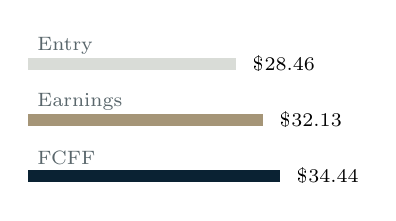
\begin{tikzpicture}[x=1cm,y=.62cm]\node[anchor=west,font=\scriptsize,text=muted]at(0,0.37){Entry};\fill[line](0,-0.13)rectangle(2.6439891831819353,0.12);\node[anchor=west,font=\scriptsize]at(2.7439891831819354,0.0){\$28.46};\node[anchor=west,font=\scriptsize,text=muted]at(0,-0.7799999999999999){Earnings};\fill[gold](0,-1.2799999999999998)rectangle(2.9849392992141803,-1.0299999999999998);\node[anchor=west,font=\scriptsize]at(3.0849392992141804,-1.15){\$32.13};\node[anchor=west,font=\scriptsize,text=muted]at(0,-1.9299999999999997){FCFF};\fill[navy](0,-2.4299999999999997)rectangle(3.2,-2.1799999999999997);\node[anchor=west,font=\scriptsize]at(3.3000000000000003,-2.3){\$34.44};\end{tikzpicture}
\par\vspace{.16cm}\smallnote{Earnings margin of safety: 11.42\%}
\end{column}
\begin{column}{.62\textwidth}
\point{We remove the tariff refund from earnings}{The refund is temporary. Negative equity also makes P/B and ROE hard to interpret.}
\point{Catalyst}{\textbf{24 November:} FY2027 guidance. We will watch PC margins, memory costs and printing.}
\point{Main risk}{Falling print sales or weaker cash flow would put pressure on earnings, dividends and buybacks.}
\end{column}\end{columns}
\source{USD per share. Cash values use our FCFF assumptions. \reportsection{2.6}; \href{https://www.hp.com/content/dam/sites/garage-press/press/press-releases/2026/q3-fy26-earnings/HP_Inc_Reports_Q3FY26_Earnings.pdf}{issuer earnings release}.}

\note{HP's guided earnings include nineteen cents from tariff refunds. We remove that amount before applying the P/E. The cash model supports the resulting value. The November 24 outlook will help us assess PC margins, memory costs and printing. Falling print sales or weaker cash flow would put pressure on dividends and buybacks. Negative book equity also makes P/B and ROE difficult to use, so we focus on earnings and cash.}
\end{frame}

\begin{frame}{Alphas and portfolio weights}

\begin{center}\large
$w_i=\frac{1}{3}\;\dfrac{\max(\alpha_i,0)/\sigma^2_{\varepsilon i}}
{\sum_j\max(\alpha_j,0)/\sigma^2_{\varepsilon j}}$
\end{center}\vspace{.10cm}
\begin{columns}[T,onlytextwidth]
\begin{column}{.59\textwidth}\tablefont
\begin{tabular}{@{}lrrr@{}}\toprule Stock & Annual alpha & Residual vol. & Fund weight\\\midrule
ADBE&12.07\%&34.81\%&4.65\%\\
KR&8.14\%&21.66\%&8.10\%\\
HRL&7.79\%&22.96\%&6.90\%\\
BMY&7.52\%&23.55\%&6.33\%\\
XOM&4.51\%&24.12\%&3.62\%\\
HPQ&7.23\%&30.08\%&3.73\%\\
\bottomrule\end{tabular}
\end{column}
\begin{column}{.36\textwidth}
\point{Kroger has the largest weight}{Kroger has relatively low residual variance, so its alpha-to-variance score is high.}
\smallnote{The 8.10\% target is just above our own 8\% preference. Stocks with negative alpha get zero weight.}
\end{column}\end{columns}
\source{Alpha = $0.5(1+k)(V/P-1)$; $k$ uses market beta. Residual risk comes from 60 monthly excess returns regressed on the SAA. The 50\% haircut is a judgement. \reportsection{3}.}

\note{We size each stock using alpha divided by residual variance, then scale the weights to one-third of the fund. Our alpha inputs come from the earnings valuations, reduced by a common fifty-percent haircut. Residual risk comes from sixty monthly excess returns against the SAA. Kroger gets the largest weight because its alpha-to-variance score is high. Its 8.10 percent weight is just above our own 8 percent preference. Capping it would change the required proportions.}
\end{frame}

\begin{frame}{Tracking error and portfolio risk}

\begin{columns}[T,onlytextwidth]
\begin{column}{.58\textwidth}
\labeltext{ANNUAL TRACKING ERROR}\par\vspace{.16cm}
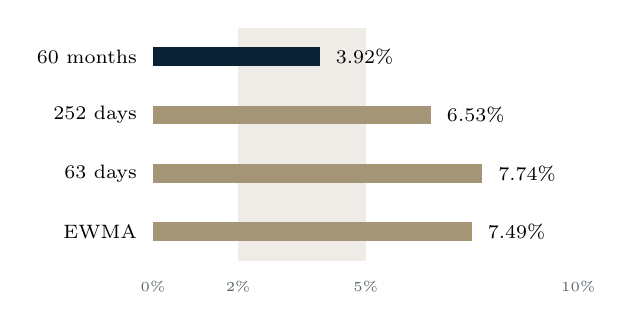
\begin{tikzpicture}[x=.54cm,y=.74cm]\fill[gold!18](2,.5)rectangle(5,-3.5);\node[anchor=east,font=\scriptsize]at(-.15,0){60 months};\fill[navy](0,-0.16)rectangle(3.91898,0.16);\node[anchor=west,font=\scriptsize]at(4.06898,0){3.92\%};\node[anchor=east,font=\scriptsize]at(-.15,-1){252 days};\fill[gold](0,-1.16)rectangle(6.53332,-0.84);\node[anchor=west,font=\scriptsize]at(6.68332,-1){6.53\%};\node[anchor=east,font=\scriptsize]at(-.15,-2){63 days};\fill[gold](0,-2.16)rectangle(7.74034,-1.84);\node[anchor=west,font=\scriptsize]at(7.89034,-2){7.74\%};\node[anchor=east,font=\scriptsize]at(-.15,-3){EWMA};\fill[gold](0,-3.16)rectangle(7.49419,-2.84);\node[anchor=west,font=\scriptsize]at(7.64419,-3){7.49\%};\node[font=\tiny,text=muted]at(0,-3.95){0\%};\node[font=\tiny,text=muted]at(2,-3.95){2\%};\node[font=\tiny,text=muted]at(5,-3.95){5\%};\node[font=\tiny,text=muted]at(10,-3.95){10\%};\end{tikzpicture}
\par\smallnote{Shaded band: the required 2--5\% range.}
\end{column}
\begin{column}{.37\textwidth}\tablefont
\begin{tabular}{@{}lrr@{}}\toprule & SAA & New\\\midrule
Volatility & 7.89\% & 9.47\%\\
1-month VaR & 3.74\% & 4.50\%\\\bottomrule\end{tabular}
\par\vspace{.35cm}\normalsize
We meet the course requirement using monthly returns. The daily estimates show higher short-term risk.
\par\vspace{.25cm}\smallnote{The original 8\% volatility target applies to the SAA.}
\end{column}\end{columns}
\source{November 2021--October 2026 monthly USD returns. Volatility is annualized; 5\% VaR assumes zero-mean normal returns. \reportsection{1.2}.}

\note{Using the required sixty monthly returns, tracking error is 3.92 percent, within the two-to-five-percent band. Portfolio volatility rises to 9.47 percent and one-month five-percent VaR to 4.50 percent of NAV. The original volatility target applies to the SAA. The daily TE estimates are higher, at roughly 6.5 to 7.7 percent. Those checks show that the monthly result can understate short-term active risk.}
\end{frame}

\begin{frame}{Backtests with different start dates}

\begin{columns}[T,onlytextwidth]
\begin{column}{.53\textwidth}
\labeltext{33-SESSION ACTIVE RETURN}\par\vspace{.10cm}
\begin{tabular}{@{}lr@{}}\toprule DBC methodology period & Mean\\\midrule
Before the change & $+0.321\%$\\
After the change & $-0.395\%$\\\bottomrule
\end{tabular}\par\vspace{.28cm}
\textbf{Later-period 95\% interval}\par\vspace{.10cm}
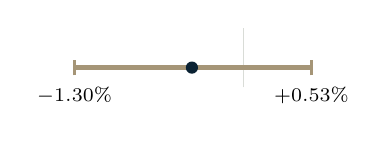
\begin{tikzpicture}[x=1.65cm,y=1cm]
\draw[line](0,-.25)--(0,.5);
\draw[gold,line width=2pt](-1.299,0)--(.525,0);
\draw[gold,line width=1pt](-1.299,-.10)--(-1.299,.10);
\draw[gold,line width=1pt](.525,-.10)--(.525,.10);
\fill[navy](-.395,0)circle(2.2pt);
\node[below,font=\scriptsize]at(-1.299,-.12){$-1.30\%$};
\node[below,font=\scriptsize]at(.525,-.12){$+0.53\%$};
\end{tikzpicture}\par\vspace{.14cm}
\smallnote{The block-bootstrap interval for mean active return includes zero.}
\end{column}
\begin{column}{.42\textwidth}
\point{217 overlapping starts}{Only 6--7 non-overlapping windows per offset; 44.2\% beat the SAA.}
\point{Monthly TE understated risk}{At 10 dates when monthly TE passed, daily TE later exceeded 5\% in 80\% of cases.}
\smallnote{We reuse today's stocks and assumptions, which limits what the backtests tell us about future returns.}
\end{column}\end{columns}
\source{DBC split: 10 November 2025. Fixed allocations and zero fees. \reportsection{1.2}; \href{https://github.com/kybeka/meridian-capital/tree/main/research/round-2}{notebook tests}.}

\note{We tested holding periods starting on different dates. DBC changed its methodology in November 2025, so we split the results around that date. In the later period, average active return is negative and 44.2 percent of windows beat the SAA. The confidence interval includes zero. Most of the 217 windows overlap, so they share many of the same days. We also reuse today's stock choices and assumptions. That limits how much these tests tell us about future returns.}
\end{frame}

\begin{frame}{Expected IR and its assumptions}

\begin{columns}[T,onlytextwidth]
\begin{column}{.48\textwidth}\tablefont
\begin{tabular}{@{}lr@{}}\toprule Annual residual IR & Estimate\\\midrule
Assuming independent residuals & 0.756\\
Including residual correlations & 0.696\\
Lower cash or earnings value & 0.564\\
Original fair values reduced 5\% & 0.426\\\bottomrule
\end{tabular}\par\vspace{.27cm}\smallnote{Annual estimates. We keep the same holdings in both valuation tests.}
\end{column}
\begin{column}{.47\textwidth}
\textbf{Fundamental Law}\par\vspace{.12cm}
{\large $IR=IC\sqrt{N}$}\par\vspace{.16cm}
With six independent ideas, an assumed $IC=0.10$ gives $IR=0.245$.
\par\vspace{.20cm}Our classroom estimate would require $IC\approx0.309$, which assumes much greater forecasting skill.
\end{column}\end{columns}
\vspace{.32cm}\small
The theoretical Sharpe gain is $\sqrt{S_B^2+IR_A^2}-S_B$, under valid alphas and optimal beta-adjusted mixing. Our stock allocation is fixed at one-third.
\source{Residual IR uses alpha per unit of residual risk; whole-fund active TE also reflects the SAA beta difference. \reportsection{3}.}

\note{The classroom residual IR is 0.756. Including residual correlations lowers it to 0.696. Using the lower cash-flow valuations lowers it again to 0.564, with the weights unchanged. The Fundamental Law helps put that in perspective. Six independent ideas with an assumed IC of 0.10 give an IR of 0.245. Reaching 0.756 would require much stronger forecasting skill. The Sharpe-gain formula also assumes valid alphas and optimal mixing, so it gives us a conditional comparison for our fixed one-third allocation.}
\end{frame}

\begin{frame}{The portfolio we entered}

\vspace{.15cm}
\begin{columns}[T,onlytextwidth]
\begin{column}{.46\textwidth}
\labeltext{INDIVIDUAL STOCKS}\par\vspace{.12cm}\bigvalue{33.33\%}\par\vspace{.20cm}
\textbf{ADBE · KR · HRL · BMY · XOM · HPQ}\par\vspace{.18cm}
Our estimated values exceed entry prices. We checked cash flow and identified news expected during the challenge.
\end{column}
\begin{column}{.47\textwidth}
\point{Monthly TE: 3.92\%}{The remaining two-thirds keep the original ETF proportions.}
\point{Main risks}{Daily risk is higher, and prices may take time to adjust. BMY has little valuation cushion; Exxon's dates are uncertain.}
\end{column}\end{columns}
\vspace{.35cm}\textbf{Questions}\hfill\href{https://kybeka.github.io/meridian-capital/materials/round-2-report.pdf}{Report}\quad\href{https://github.com/kybeka/meridian-capital/tree/main/research/round-2}{Code and model}
\source{Entered 7 November at 6 November closing prices. The holdings and quantities match the submitted report.}

\note{This is the portfolio we entered: six stocks, funded by proportional ETF sales, with monthly TE of 3.92 percent. The estimated values and catalysts explain why we chose them. The daily risk checks and backtests show why the outcome is uncertain. We'll watch the company results and reconsider the cases at the next scheduled rebalance. The backup slides contain the cash models, catalyst dates and trade list for questions.}
\end{frame}

\appendix
\setbeamertemplate{footline}{\hspace{1.05cm}\begin{minipage}{\dimexpr\paperwidth-2.1cm\relax}{\color{line}\hrule height .3pt}\vspace{3pt}{\fontsize{5.7}{7}\selectfont\color{muted}MERIDIAN CAPITAL\enspace ·\enspace AMC 2026\hfill Backup \insertframenumber}\vspace{5pt}\end{minipage}}

\begin{frame}{Cash-flow assumptions}

\tablefont\begin{tabularx}{\textwidth}{@{}Xrrrrr@{}}\toprule
Stock & 5-year growth & Terminal growth & WACC & FCFF value & Lower value\\\midrule
ADBE&8.0\%&3.0\%&13.08\%&\$271.14&\$271.14\\
KR&3.0\%&2.0\%&6.31\%&\$87.45&\$78.00\\
HRL&2.0\%&2.0\%&6.20\%&\$31.49&\$25.16\\
BMY&0.0\%&0.0\%&5.83\%&\$65.50&\$65.50\\
XOM&2.0\%&2.0\%&5.83\%&\$213.08&\$180.00\\
HPQ&4.0\%&3.0\%&10.94\%&\$34.44&\$32.13\\
\bottomrule\end{tabularx}\par\vspace{.20cm}
\small Lower value = min(earnings, FCFF). We use the same debt policy in FCFF and FCFE. Terminal value is a large part of the result.
\par\vspace{.25cm}\small
We deduct SBC and adjust for cash, debt and minority interests. The values depend on our starting cash flow, growth and discount rates.
\source{Values in USD per share. \reportsection{2.7}; companion notebook.}

\note{We use the same debt policy in the FCFF and FCFE models so that the values are comparable. We take the lower of the earnings and cash values for the conservative check. We deduct stock compensation and adjust for cash, debt and minority interests. The starting cash flow, growth rates, discount rates and terminal value all matter to the result.}
\end{frame}

\begin{frame}{Growth and holding-period assumptions}

\begin{columns}[T,onlytextwidth]
\begin{column}{.42\textwidth}\tablefont
\begin{tabular}{@{}lrr@{}}\toprule Stock & Base growth & Implied growth\\\midrule
ADBE&8.0\%&4.89\%\\
KR&3.0\%&0.70\%\\
HRL&2.0\%&-0.59\%\\
BMY&0.0\%&-0.95\%\\
XOM&2.0\%&0.29\%\\
HPQ&4.0\%&1.57\%\\
\bottomrule\end{tabular}\par\vspace{.20cm}
\smallnote{Cash growth needed over five years to justify the entry price, using the lower valuation and keeping other inputs fixed.}
\end{column}
\begin{column}{.53\textwidth}\tablefont
\textbf{Adobe: annual cash-based IRR}\par\vspace{.15cm}
\begin{tabularx}{\linewidth}{@{}Xr@{}}\toprule Scenario & IRR\\\midrule
1-year convergence & 28.17\%\\
3-year convergence & 17.21\%\\
3-year discount persists & 12.43\%\\\bottomrule\end{tabularx}
\par\vspace{.20cm}\normalsize
If the price takes longer to reach our value, the annual return is lower. The discount may also remain.
\end{column}\end{columns}
\source{These scenarios use holding periods longer than the challenge. The 50\% alpha haircut is a judgement. \reportsection{2.7}.}

\note{Implied growth is the growth rate that would justify the entry price with the other inputs fixed. It depends on our cash-flow and discount-rate assumptions. We also tested what happens if the price takes longer to reach our value. Adobe's annual return is lower when convergence takes three years instead of one, and the discount may remain. These are longer holding periods than the challenge.}
\end{frame}

\begin{frame}{Cash flow and value-trap risks}

\tablefont\begin{tabularx}{\textwidth}{@{}lrrrX@{}}\toprule
 & FCF margin & Prior mean & Peer median & Main warning\\\midrule
ADBE & 41.4\% & 38.1\% & 34.7\% & Buybacks, leverage and AI competition\\
KR & 2.3\% & 1.4\% & 2.1\% & Payouts exceed cash available without new debt\\
HRL & 4.4\% & 7.3\% & 8.7\% & Thin dividend cover; acquisition debt\\
BMY & 26.7\% & 27.6\% & 25.6\% & Patent expiry and replacement medicines\\
XOM & 7.3\% & 11.2\% & 12.3\% & Cycle dependence and lower cash generation\\
HPQ & 5.1\% & 5.8\% & 7.5\% & Falling print sales and high payouts\\\bottomrule
\end{tabularx}\par\vspace{.20cm}
\small Annual comparisons use the latest full year, up to three earlier years and the named peer groups. The cash valuations use the separately stated TTM or normalized inputs.
\source{\reportsection{2}; annual quality inputs and peer comparisons in the notebooks.}

\note{We checked whether the low multiples could reflect lasting problems in earnings or cash flow. Adobe and Kroger have stronger FCF margins than their historical and peer comparisons. Hormel needs a recovery, BMY needs new medicines to replace lost sales, and Exxon depends on the oil cycle. HP faces falling print sales. The annual comparisons use different periods from the TTM or guidance inputs in the cash models.}
\end{frame}

\begin{frame}{Catalysts and the challenge calendar}

\tablefont\begin{tabularx}{\textwidth}{@{}lXl@{}}\toprule
Date & Event and what we will watch & Timing\\\midrule
24 November & HP results and FY2027 guidance & Confirmed\\
28--29 November & Next scheduled portfolio rebalance & Course calendar\\
3 December & Kroger results: sales, fulfillment costs and cash & Confirmed\\
3 December & Hormel outlook: recovery and dividend coverage & Confirmed\\
9 December & Adobe outlook: renewals, pricing and paid AI demand & Confirmed\\
12--15 December & BMY data at ASH & Meeting dates fixed\\
Q4 / year-end & BMY readouts; Exxon Uaru and corporate plan & No fixed day\\
27 December & Challenge cutoff used in our analysis & Portfolio horizon\\\bottomrule
\end{tabularx}\par\vspace{.20cm}
\small Kroger and Hormel together account for about 15\% of NAV and report on the same day. Several events fall after the next rebalance. Events without fixed dates could miss the cutoff.
\source{As recorded in the submitted report, sections 2--3. Annual alpha assumptions extend beyond the current holding period.}

\note{HP reports first. Kroger and Hormel both report on December 3, so about fifteen percent of NAV faces company news on the same day. Most catalysts fall after the next rebalance. BMY and Exxon have events expected by year-end without confirmed dates, which could put them beyond December 27. The news could also disappoint and move prices against us.}
\end{frame}

\begin{frame}{Why we chose six stocks}

\begin{center}\begin{tabular}{@{}lrr@{}}\toprule
 & Five-stock IR maximum & Chosen six stocks\\\midrule
Forecast residual IR & 0.698 & 0.696\\
Recent daily TE & 8.68\% & 7.74\%\\
Largest stock target & 9.09\% & 8.10\%\\\bottomrule
\end{tabular}\end{center}\vspace{.25cm}
\small We compared all 420 three-to-six-stock combinations within nine researched positive-alpha cases. FDS, INTU and GILD were alternatives.
\par\vspace{.25cm}With six stocks, forecast IR is almost unchanged, while recent TE and the largest stock weight are lower. The largest stock still exceeds our additional 8\% preference.
\source{We compare the stocks we researched using the same weighting rule. \reportsection{2.8}; main notebook.}

\note{We compared combinations of three to six stocks from the nine names we researched. The five-stock maximum has an IR of 0.698, against 0.696 for our six. That is a small difference. The six-stock portfolio has lower recent daily TE and a smaller largest position. We preferred that tradeoff, while recognizing that the largest stock still exceeds our own preference.}
\end{frame}

\begin{frame}{Final holdings and trades}

\fontsize{8}{10.2}\selectfont
\begin{tabularx}{\textwidth}{@{}Xrrrr@{}}\toprule
Bloomberg ID & Shares & Entry price & NAV weight & Trade shares\\\midrule
SPY US Equity & 22,964 & \$735.29 & 17.39\% & -11,205\\
EEMV US Equity & 89,717 & \$69.71 & 6.44\% & -43,893\\
DBC US Equity & 553,213 & \$31.54 & 17.97\% & -245,543\\
SCHD US Equity & 60,380 & \$35.17 & 2.19\% & -35,108\\
VGSH US Equity & 55,948 & \$57.86 & 3.33\% & -30,723\\
STIP US Equity & 186,996 & \$100.51 & 19.35\% & -101,634\\
ADBE US Equity & 18,865 & \$239.30 & 4.65\% & +18,865\\
KR US Equity & 116,215 & \$67.70 & 8.10\% & +116,215\\
HRL US Equity & 305,167 & \$21.95 & 6.90\% & +305,167\\
BMY US Equity & 99,004 & \$62.14 & 6.33\% & +99,004\\
XOM US Equity & 21,201 & \$165.87 & 3.62\% & +21,201\\
HPQ US Equity & 127,276 & \$28.46 & 3.73\% & +127,276\\
\bottomrule\end{tabularx}\par\vspace{.18cm}
\smallnote{USD throughout. Entry: 7 November; price: 6 November close. Cash: \$116.05. NAV: \$97,115,068.58. Securities: \$97,114,952.53. Stocks: 33.33320\% of NAV.}
\source{Positive trades are purchases; negative trades are sales. The extra SPY and Adobe shares are included. \reportsection{5}.}

\note{These are the shares and trades in the submitted report. Prices are the November 6 close, and the entry date is November 7. Rounding to whole shares leaves the stock allocation 130.49 dollars below the exact one-third budget. The extra SPY and Adobe shares are included. The remaining cash is 116.05 dollars.}
\end{frame}

\begin{frame}{Sources and methods}

\point{Company information}{Issuer releases, financial statements, investor calendars and the peer comparisons archived with the notebooks. Stock-specific links appear on the six company slides.}
\point{Market and risk inputs}{Public prices and total returns; FRED Treasury rates. Monthly calibration: November 2021--October 2026. Entry prices: 6 November 2026 close.}
\point{Calculations and data}{\href{https://github.com/kybeka/meridian-capital/tree/main/research/round-2}{Two executed notebooks, saved inputs, result tables and Excel model}. The \href{https://kybeka.github.io/meridian-capital/materials/round-2-report.pdf}{submitted report} and portfolio description use the same NAV and quantities.}
\source{The company information, assumptions and event dates are the same as in our submitted report.}

\note{The two notebooks and Excel model contain the inputs, assumptions and calculations. The report has the company analysis and sources. Market beta is used in the discount rate, while the SAA regression gives us residual risk. We also distinguish forecast residual IR from historical active returns, and the monthly course requirement from the extra daily checks.}
\end{frame}
\end{document}
